\documentclass[12pt]{article}


\RequirePackage{lipsum}
\RequirePackage{array}
\RequirePackage{colortbl}
\RequirePackage{chemfig}
\usepackage{mathtools}
\usepackage{pdfpages}
\usepackage{graphicx}
\usepackage{titling}
\usepackage[ddmmyyyy]{datetime}
\renewcommand{\dateseparator}{.}
\usepackage{float}
\usepackage{setspace}
\onehalfspacing
\usepackage{amsmath}
\usepackage{pdflscape}
\usepackage{rotating}
\usepackage[backend=biber]{biblatex}
\addbibresource{uni.bib}
\renewcommand{\contentsname}{Innhold}


\usepackage{booktabs}
\usepackage{caption}
\captionsetup[table]{name=Tabell}
\captionsetup[figure]{name=Figur}

\usepackage{hyperref}
\hypersetup{
	colorlinks=true,
	citecolor = black,
	linkcolor=black,
	filecolor=black,      
	urlcolor=black,
	pdftitle={Sharelatex Example},
	pdfpagemode=FullScreen,}


\author{\\
\includegraphics[scale=0.8]{ntnu-logo.jpg}
		\\\\Edvard Kaldhusdal
		\\Jan Olav Løveseter
		\\Lars Hammer
		\\Åsmund Ødegård Pettersen\\
		\\}
\title{PAPIRBRO}
\date{\today}
\usepackage{geometry}



\begin{document}



\begin{titlingpage}
\maketitle
\end{titlingpage}

\thispagestyle{empty}
\pagebreak
\tableofcontents
\thispagestyle{empty}
\pagebreak
\clearpage
\pagenumbering{arabic}

 
\section{Del 1}
\subsection{Innledning}
4 studenter satt sammen og løste en øving i konstruksjonsteknikk, da det oppstod et spørsmål i gruppen. Hva er mest avgjørende for bæreevnen til en liten papirbro? Det ble bestemt at dette skulle testes for å sjekke hva som påvirker broens bæreevne mest. Målet er å planlegge, gjennomføre og diskutere et $2^k$ forsøk og finne ut hvordan forskjellige faktorer påvirker broens bæreevne. Studentene involvert i forsøket går andre året på byggingeniør og har litt kunnskaper om hvordan forskjellige laster påvirker konstruksjoner og hvilke muligheter man har for å styrke en konstruksjon. 

Ved å legge lader og mynter oppå broen måles det hvor mye den tåler før kollaps. Faktorene i forsøket er tykkelsen på papiret, om broen har kantene brett eller ikke og lengden på brua.


\pagebreak
\subsection{Planlegging av forsøket}
Det ble valgt et oppsett som gjør at alle variabler kan måles. For å få et bredt nok grunnlag gjøres det målinger med gjentak slik at det totalt blir 16 målinger.

Responsen i forsøket måles ved å telle antall mynter, eventuellt lader, broen klarer å bære før den kollapser. På grunn av at myntene veier mer enn 1 gram vil det bli noe avvik fra faktisk bæreevne og testet bæreevne.

Det hadde vært mulig å velge andre faktorer i forsøket, men hovedsaklig ville disse innebært en annen form for bretting av papiret.

Ettersom det er stor forskjell på tykkelsen til papirene kan det se ut som om dette vil får en stor innvirkning på bæreevnen. Dette kombinert med brett på papiret vil nok gi den største effekten på responsen.

% Table generated by Excel2LaTeX from sheet 'Sheet1'
\begin{table}[H]
  \centering
  \caption{Faktorer og nivå.}
    \begin{tabular}{rlll}
    \toprule
    \multicolumn{1}{l}{\textbf{Nivå}} & \textbf{Tykkelse} & \textbf{Brett} & \textbf{Lengde} \\
    \midrule
    1     & Tykk  & Brett & Lang (15cm) \\
    -1    & Tynn  & Ikke brett & Kort (10cm) \\
    \bottomrule
    \end{tabular}%
  \label{tab:tab1}%
\end{table}%

Som tabell \ref{tab:tab1} viser blir det valgt to nivåer for hver faktor. Tykkelsen på papiret settes til enten tykk eller tynn, hvor vekten på arkene er henholdsvis $300g$ og $80g$. Den andre faktoren har nivåene $Brett$ og $Ikke\ brett$, hvor broene med brett får hver av langsidene brettet opp. Den siste faktoren er broens lengde og deles opp i nivåene $Lang\ (15cm)$ og $Kort\ (10cm)$. Dette reguleres ved å endre avstanden mellom stablene med papirark som støtter opp broen på hver side. Forsøket får en "$2^3$ med gjentak" organisering, ettersom forsøket gjøres to ganger.

% Table generated by Excel2LaTeX from sheet 'Ark1'
\begin{table}[H]
  \centering
  \caption{Forsøksplan med randomisert rekkefølge.}
    \begin{tabular}{rrrrrr}
    \toprule
    \multicolumn{1}{l}{\textbf{StdOrder}} & \multicolumn{1}{l}{\textbf{RunOrder}} & \multicolumn{1}{l}{\textbf{Tykkelse}} & \multicolumn{1}{l}{\textbf{Brett}} & \multicolumn{1}{l}{\textbf{Lengde}} & \\
    \midrule
    2     & 1     & 1     & -1    & -1  \\
    \midrule
    14    & 2     & 1     & -1    & 1   \\
    \midrule
    7     & 3     & -1    & 1     & 1   \\
    \midrule
    6     & 4     & 1     & -1    & 1   \\
    \midrule
    8     & 5     & 1     & 1     & 1   \\
    \midrule
    15    & 6     & -1    & 1     & 1   \\
    \midrule
    4     & 7     & 1     & 1     & -1   \\
    \midrule
    10    & 8     & 1     & -1    & -1  \\
    \midrule
    16    & 9     & 1     & 1     & 1   \\
    \midrule
    13    & 10    & -1    & -1    & 1    \\
    \midrule
    5     & 11    & -1    & -1    & 1    \\
    \midrule
    12    & 12    & 1     & 1     & -1   \\
    \midrule
    3     & 13    & -1    & 1     & -1   \\
    \midrule
    9     & 14    & -1    & -1    & -1   \\
    \midrule
    1     & 15    & -1    & -1    & -1   \\
    \midrule
    11    & 16    & -1    & 1     & -1   \\
    \bottomrule
    \end{tabular}%
  \label{tab:tab2}%
\end{table}%

Målingene utføres ved å legge en og en mynt på broen til den kollapser. Antallet mynter før kollapsen blir deretter telt opp og responsverdien regnes ut. Randomiseringen gjøres ved hjelp av Minitab.

\pagebreak
\subsection{Gjennomføring av forsøket}

Først ble papirbroene laget, dette ble gjort ved å klippe opp flere biter av tykt papir og tynt papir med dimensjoner $20 cm * 5 cm$, noen av disse papirbitene ble brettet opp på sidene for å få med en faktor som forventes å styrke broene. To stabler med ark i lik høyde ble satt opp på hver side av broene, papirbroene ble lagt fra kant til kant for å danne en bro mellom stablene. Målingene ble først gjort med kort lengde og deretter lang lengde. For å måle bæreevnen ble det lagt på mynter og eventuell lader til broen kollapset. Antall mynter og eventuell lader ble notert for å senere regne om til gram. 

 Målingene som ble gjort gikk ikke helt etter planen, ettersom det måtte brukes en lader for å få nok vekt til å kollapse enkelte broer. Randomiseringen av målingene gikk etter planen. Observasjonene var uavhengige av hverandre.


% Table generated by Excel2LaTeX from sheet 'Ark1'
\begin{table}[H]
  \centering
  \caption{Forsøksplan med randomisert rekkefølge og responsverdi.}
    \begin{tabular}{rrrrrr}
    \toprule
    \multicolumn{1}{l}{\textbf{StdOrder}} & \multicolumn{1}{l}{\textbf{RunOrder}} & \multicolumn{1}{l}{\textbf{Tykkelse}} & \multicolumn{1}{l}{\textbf{Brett}} & \multicolumn{1}{l}{\textbf{Lengde}} & \multicolumn{1}{l}{\textbf{Gram}} \\
    \midrule
    2     & 1     & 1     & -1    & -1    & 87 \\
    \midrule
    14    & 2     & 1     & -1    & 1     & 13,05 \\
    \midrule
    7     & 3     & -1    & 1     & 1     & 21,75 \\
    \midrule
    6     & 4     & 1     & -1    & 1     & 16,05 \\
    \midrule
    8     & 5     & 1     & 1     & 1     & 169 \\
    \midrule
    15    & 6     & -1    & 1     & 1     & 17,4 \\
    \midrule
    4     & 7     & 1     & 1     & -1    & 243,05 \\
    \midrule
    10    & 8     & 1     & -1    & -1    & 83,35 \\
    \midrule
    16    & 9     & 1     & 1     & 1     & 155,95 \\
    \midrule
    13    & 10    & -1    & -1    & 1     & 1,05 \\
    \midrule
    5     & 11    & -1    & -1    & 1     & 0,8 \\
    \midrule
    12    & 12    & 1     & 1     & -1    & 222,95 \\
    \midrule
    3     & 13    & -1    & 1     & -1    & 30,45 \\
    \midrule
    9     & 14    & -1    & -1    & -1    & 4,35 \\
    \midrule
    1     & 15    & -1    & -1    & -1    & 4,35 \\
    \midrule
    11    & 16    & -1    & 1     & -1    & 39,6 \\
    \bottomrule
    \end{tabular}%
  \label{tab:tab3}%
\end{table}%

\pagebreak
\subsection{Analyse av målingene}

\begin{figure}[H]
      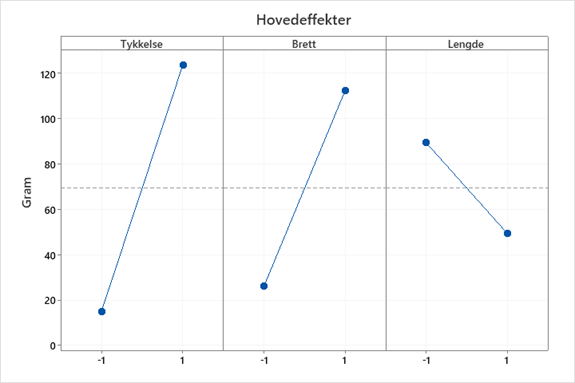
\includegraphics[width=\linewidth]{Figur 1.png}
      \caption{Hovedeffekter}
      \label{fig:fig1}
\end{figure}
    
\hyperref[fig:fig1]{Figur 1} viser hovedeffekten til hver stokastiske variabel ved lav(-1) og høy(1) verdi. Hovedeffekten finner man ved å regne ut gjennomsnittet ved henholdsvis lav og høy verdi. Grafen viser at den variabelen med størst differanse mellom lav og høy er den variabelen som gir størst effekt på resultatet, i dette tilfellet broens bæreevne(g).
Tykkelsen på papiret har størst effekt på bæreevnen. Om broen har en brett eller ikke har nest mest effekt, mens lengden på broen har minst å si for broens bæreevne.\cite{1}

\begin{figure}[H]
    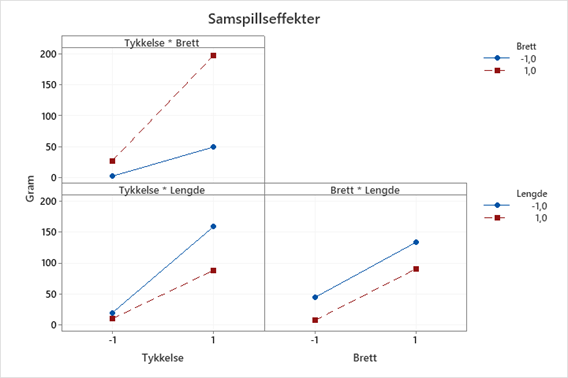
\includegraphics[width=\linewidth]{Figur 2.png}
    \caption{Samspillseffekter}
    \label{fig:fig2}
\end{figure}

\hyperref[fig:fig2]{Figur 2} viser oss samspillseffektene. Samspillseffekten sier noe om hvor mye to faktorer samhandler med hverandre. Hvis to faktorer samhandler vil de krysse hverandre, altså er de ikke-parallelle.
Grafene som viser $Tykkelse*Brett$ på \hyperref[fig:fig2]{figur 2} har to ikke-parallelle linjer. Dette vil si at disse to variablene har en samspillseffekt. Den blå linjen viser bæreevnen når tykkelsen går fra lav til høy, mens brett er på konstant lav verdi. Den stiplete røde linjen viser tykkelsen fra lav til høy mens brett har konstant høy verdi. 
Forskjellen i bæreevnen til de to linjene ved lav tykkelse er ikke stor, men ved høy tykkelse ser man at bæreevnen nesten firedobles. Dette kan tolkes som at samhandlingen mellom $Tykkelse*Brett$ har stor effekt på resultatet. Linjene i plottet som viser $Tykkelse*Lengde$ er heller ikke parallelle. Dette samspillet vil også ha en effekt på bæreevnen til broen, men det er ikke like «imponerende» som ved $Tykkelse*Brett$.  


Hvis to linjer er parallelle så er det ikke noe samspillseffekt mellom faktorene. Plottet til $Brett*Lengde$ viser to linjer som er parallelle, altså øker linjene i takt med hverandre når Brett går fra lav til høy uansett om Lengden  høy eller lav.\cite{1}



\begin{figure}[H]
    \centering
    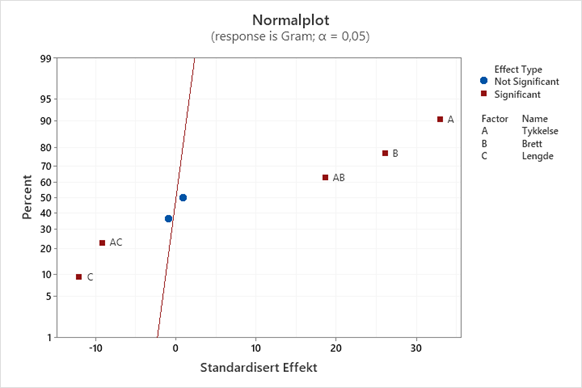
\includegraphics[scale=0.7]{Figur 3.png}
    \caption{Normalplott}
    \label{fig:fig3}
\end{figure}

\begin{figure}[H]
    \centering
    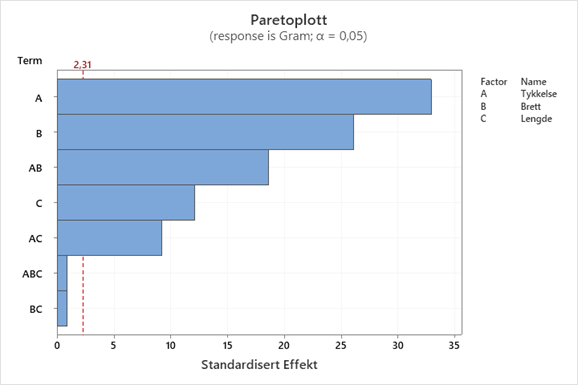
\includegraphics[scale=0.7]{Figur 4.png}
    \caption{Paretoplott}
    \label{fig:fig4}
\end{figure}
\clearpage

For å finne ut hvilke effekter som er signifikante bruker man normalplott og Paretoplott som vist i figur \hyperref[fig:fig3]{3} og \hyperref[fig:fig4]{4}. Signifikansnivået settes til 0.05 som betyr at det er 5\% sjanse for at en gyldig nullhypotese forkastes. Det er enighet om at dette signifikansnivået er tilstrekkelig for dette forsøket.
Begge disse grafene tar utgangspunkt i at hvert resultat er normalfordelt og uavhengig av hverandre med samme varians. Det blir benyttet en hypotesetest for å sjekke om en faktor er signifikant eller ikke. Nullhypotesen viser at ingen av faktorene har noe effekt, og som følge av dette blir normalfordelingen $N(0 , \frac{4\sigma^2}{n})$, hvor $\frac{4\sigma^2}{n}$ er variansen til en vilkårlig faktor. 
Nullhypotesen er som følger: Estimatet av en vilkårlig faktor er null.
Den alternative hypotesen blir: Estimatet av en vilkårlig faktor er ulik null. 

I normalplottet estimerer man en fordelingsfunksjon fra verdiene til faktorene, som er gitt ved tykkelse, brett og lengde, mens verdien er bæreevne. Denne blir standardisert til standard normalfordeling. Da vil man få $G(z)=\frac{y-\mu}{\sigma}$ ut ifra normalfordelingens fordelingsfunksjon. Dette medfører at z blir en lineær funksjon av $y$, som betyr at effekter som ligger nært denne linjen ikke er signifikante med tanke på nullhypotesen. Effekter som ligger langt unna vil følge den alternative hypotesen og dermed bli signifikante.\cite{1}
\hyperref[fig:fig3]{Figur 3} viser variablene plottet sammen med den lineære linjen definert tidligere. Fra dette kan det konkluderes at faktorene blir:

% Table generated by Excel2LaTeX from sheet 'Sheet1'
\begin{table}[htbp]
  \centering
  \caption{Signifikante og ikke-signifikante faktorer}
    \begin{tabular}{rl}
    \toprule
    \multicolumn{1}{l}{\textbf{Ikke-signifikante}} & \textbf{Signifikante} \\
    \midrule
    \multicolumn{1}{l}{$ABC=Tykkelse*Brett*Lengde$} & $A=Tykkelse$ \\
    \multicolumn{1}{l}{$BC=Brett*Lengde$} & $B=Brett$ \\
          & $C=Lengde$ \\
          & $AB=Tykkelse*Brett$ \\
          & $AC=Tykkelse*Lengde$ \\
          \bottomrule
    \end{tabular}%
  \label{tab:tabell2}%
\end{table}%



I blant annet Paretoplottet (\hyperref[fig:fig4]{figur 4}) blir Lenths metode brukt. Metoden går ut på at man skal finne et estimat for faktorenes standardavvik. Dette blir gjort ved å ta medianen av faktorenes tallverdi, populært kalt Lenths PSE. Med Lenths metode benytter man seg også av hypotesetesting, som går ut på å forkaste nullhypotesen hvis en tallverdi er større eller lik C*PSE. Der C er en variabel som varierer for signifikansnivå og antall forsøk. 
Resultatet av C*PSE er den stiplete røde linjen med verdi 2,31 vist i \hyperref[fig:fig4]{figur 4}. Alle verdier som er høyere enn 2,31 vil være signifikante fordi nullhypotesen kan forkastes. Resultatet av Lenths metode i Minitab er noe høyere enn den reelle verdien. Hvis noen faktorer lå nærmere 2,31 kunne man regnet den reelle Lenths verdien og senket kravet for signifikans. I plottet (\hyperref[fig:fig4]{figur 4}) ligger faktorene så langt unna 2,31 det ikke blir flere signifikante faktorer ved ny utregning av Lenths verdi.\cite{1}


Både Normalplottet og Paretoplottet viser at A, B, C, AB, AC er signifikante faktorer når signifikansnivået er 5\%.


\begin{equation}
\begin{aligned}
\centering
Gram &= {69,38 + 54,42*(Tykkelse) + 43,13*(Brett) 
    \\&- 20,00*(Lengde)+ 30,80*(Tykkelse*Brett) 
    \\&- 15,28*(Tykkelse*Lengde)-1,49*(Brett*Lengde)
    \\&+1,52*(Tykkelse*Brett*Lengde)}
        \label{lig1}
\end{aligned}
\end{equation}

\hyperref[lig1]{Ligning 1} viser regresjonsligningen for forsøket. Regresjonsligningen brukes for å regne ut bæreevnen til broen når faktorene er på sin lav eller høy verdi. Ved å erstatte faktorene i ligningen med enten -1 eller 1, kan det regnes ut et estimat for resultatet.
Ligningen kan forkortes til å kun inneholde de signifikante faktorene, ettersom de faktorene som ikke er signifikante vil ha liten effekt på broens bæreevnen.\cite{1}


Den forkortede ligningen for broens bæreevne blir dermed:

\begin{equation}
    \begin{aligned}
    \centering
Gram = {}& {69,38 + 54,42*(Tykkelse)\\ 
         &+ 43,13*(Brett) - 20,00*(Lengde) \\
         &+ 30,80*(Tykkelse*Brett)\\
         &- 15,28*(Tykkelse*Lengde)}
         \label{lig2}
    \end{aligned}
\end{equation}
\\
Figur 5 til 8 viser residualer som brukes for å forsikre at modellen er tilstrekkelig for forsøket og representerer avvik fra regresjonsligningen. Residualen regnes ut ved å ta svaret fra ligning \hyperref[lig1]{(1)} og trekke dette fra det målte resultatet. Svaret er da residualen for det unike forsøket.\cite{1}

\begin{figure}[H]
    \centering
    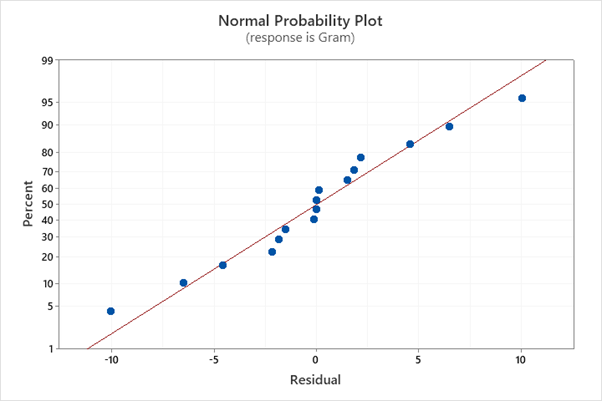
\includegraphics[width=\linewidth]{Figur 5.png}
    \caption{Normal sannsynlighetsplott}
    \label{fig:fig5}
\end{figure}

Normal sannsynlighetsplottet i \hyperref[fig:fig5]{figur 5} forteller oss om effekten av faktoren har samme varians. Hvis dette stemmer vil residualene ligge tilnærmet langs den lineære linjen i \hyperref[fig:fig5]{figur 5}, som er tilfellet i dette forsøket. Det kan derfor konkluderes med at normal sannsynlighetsplottet er korrekt.\cite{1}


\begin{figure}[H]
    \centering
    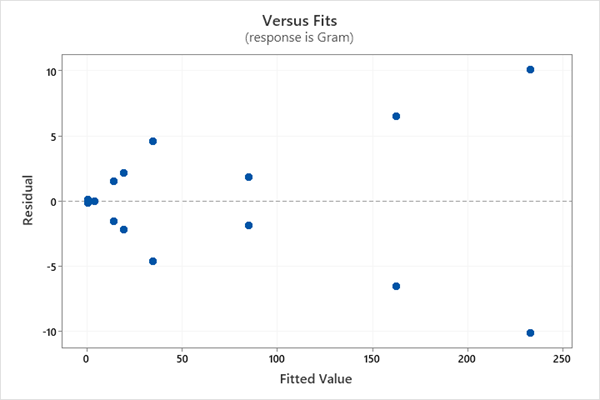
\includegraphics[width=\linewidth]{Figur 6.png}
    \caption{Versus fits diagram}
    \label{fig:fig6}
\end{figure}

Versus fits diagrammet viser et plott av residualer i forhold til verdien sin. Diagrammet er symmetrisk om $x$-aksen til $y=0$. Dette forsterker troen på et godt gjennomført forsøk.\cite{1}

\begin{figure}[H]
    \centering
    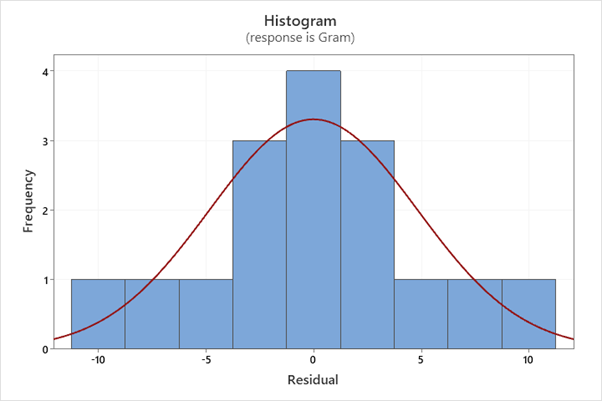
\includegraphics[width=\linewidth]{Figur 7.png}
    \caption{Histogram}
    \label{fig:fig7}
\end{figure}

I \hyperref[fig:fig7]{figur 7} forventes noe som ligner på en normalfordeling. Det er tegnet en rød hjelpelinje som viser hvordan forsøket ville blitt med n antall gjentak. Kurven ser ut til å bli tilnærmet normalfordelt, noe som forsterker resultatet.\cite{1}  

\begin{figure}[H]
    \centering
    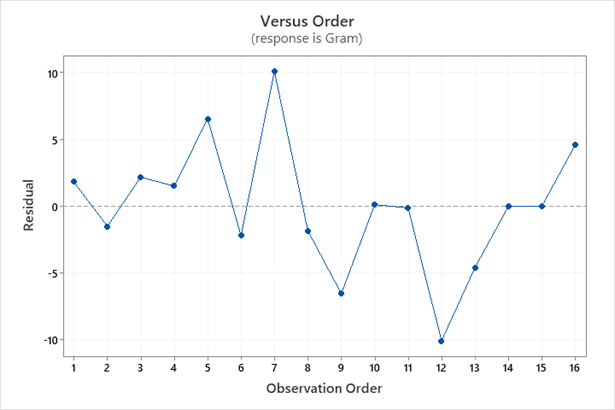
\includegraphics[width=\linewidth]{Figur 8.png}
    \caption{Versus order diagram}
    \label{fig:fig8}
\end{figure}

Versus order diagrammet i \hyperref[fig:fig8]{figur 8} viser rekkefølgen av residualer og tilhørende verdi. Diagrammet sjekkes for store avvik eller om det har oppstått noen unormale verdier. Det er ingen mistanker om store feil i dette plottet.\cite{1}


\clearpage
\subsection{Konklusjon}
Analysen av plottene i de fire første figurene viser hvilke faktorer som er signifikante og hvilke som ikke er det. Konklusjonen, som vist i \hyperref[tab:tabell2]{tabell 2}, er at A, B, C, AB og AC er signifikante faktorer når signifikansnivået er 5\%, mens BC og ABC ikke er signifikante faktorer. 

Residualene i figur 5-8 ble analysert og viste at alle fire diagrammene er normale. Dette betyr at det ikke har skjedd noen store feil i analysen av resultatene og det konkluderes med at resultatene er riktige.


\renewcommand\refname{Referanser}
\begin{thebibliography}{}
\bibitem{forelesninger}
Kjell Arnesen, videoforelesninger uke 10 og 11.


\end{thebibliography}



\pagebreak
\section{Del 2}
\subsection{Innledning}
I denne delen av prosjektet ble det fokusert på statistisk kvalitetskontroll. Det ble foretatt kontrollmålinger på en fiskeforedlingsbedrift, for å sikre at vekten på fisken som selges til kundene er korrekt.


\subsection{Resultater og konklusjon}

\begin{table}[H]
\centering
\caption{Vekt på fiskefiletene}
\begin{tabular}{lrrrrr}
\toprule
{} &           0 &           1 &           2 &           3 &           4 \\
\midrule
0 &  101.624345 &   99.388244 &   99.471828 &   98.927031 &  100.865408 \\
1 &   97.698461 &  101.744812 &   99.238793 &  100.319039 &   99.750630 \\
2 &  101.462108 &   97.939859 &   99.677583 &   99.615946 &  101.133769 \\
3 &   98.900109 &   99.827572 &   99.122142 &  100.042214 &  100.582815 \\
4 &   98.899381 &  101.144724 &  100.901591 &  100.502494 &  100.900856 \\
5 &   99.316272 &   99.877110 &   99.064231 &   99.732112 &  100.530355 \\
6 &   99.308339 &   99.603246 &   99.312827 &   99.154794 &   99.328754 \\
7 &   99.987335 &   98.882690 &  100.234416 &  101.659802 &  100.742044 \\
8 &   99.808164 &   99.112371 &   99.252842 &  101.692455 &  100.050808 \\
9 &   99.363004 &  100.190915 &  102.100255 &  100.120159 &  100.617203 \\
\bottomrule
\end{tabular}

\label{tab:tab5}
\end{table}



\begin{figure}[H]
    \centering
    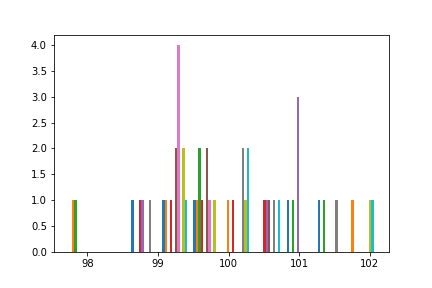
\includegraphics[scale= 1]{norm.png}
    \caption{Normalfordeling av fiskefiletene}
    \label{fig:fig9}
\end{figure}

\hyperref[fig:fig9]{Figur 9} er en visualisering av dataen gitt i \hyperref[tab:tab5]{tabell 5}. Diagrammet viser at målingene av fiskefiletene danner en normalfordelt distribusjon.


\begin{table}[H]
    \centering
    \caption{Gjennomsnittet av hver måling.}
\begin{tabular}{lr}
\toprule
{} &           0 \\
\midrule
0 &  100.055371 \\
1 &   99.750347 \\
2 &   99.965853 \\
3 &   99.694970 \\
4 &  100.469809 \\
5 &   99.704016 \\
6 &   99.341592 \\
7 &  100.301257 \\
8 &   99.983328 \\
9 &  100.478307 \\
\bottomrule
\end{tabular}
    
    \label{tab:tab6}
\end{table}

\begin{figure}[H]
    \centering
    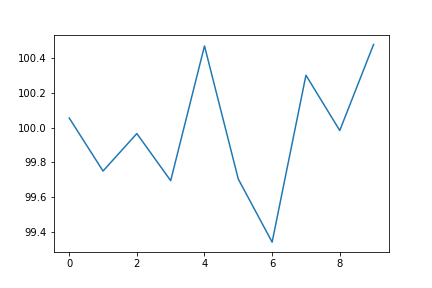
\includegraphics[scale = 1]{gj_plot.png}
    \caption{Gjennomsnittet av hver måling.}
    \label{fig:fig10}
\end{figure}

Gjennomsnittet til gjennomsnittet av hver måling ble regnet ut til  $\overline{\overline{x}}=99.974485$.



\begin{table}[H]
    \centering
    \caption{Standardavviket av hver måling.}
\begin{tabular}{lr}
\toprule
{} &         0 \\
\midrule
0 &  1.137604 \\
1 &  1.480981 \\
2 &  1.406502 \\
3 &  0.686725 \\
4 &  0.907615 \\
5 &  0.564194 \\
6 &  0.162369 \\
7 &  1.019226 \\
8 &  1.030598 \\
9 &  1.013012 \\
\bottomrule
\end{tabular}
    \label{tab:tab7}
\end{table}



\begin{figure}[H]
    \centering
    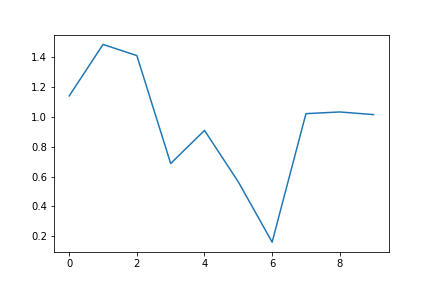
\includegraphics[scale = 1]{avvik1.png}
    \caption{Standardavviket av hver måling.}
    \label{fig:fig11}
\end{figure}
Gjennomsnittet til standardavvikene ble regnet ut til $\overline{\overline{s}}=0.940883$.

Utregning av øvre- og nedre kontrollgrense (ØKG og NKG)\cite{1}:

\begin{equation}
\centering
\begin{aligned}
ØKG & = {\overline{\overline{x}}+\frac{3*\overline{\overline{s}}}{\sqrt{10}}}=100.867085\\
NKG & = {\overline{\overline{x}}-\frac{3*\overline{\overline{s}}}{\sqrt{10}}}=99.081886  
\end{aligned}
\end{equation}

Utregning av øvre- og nedre varselgrense (ØVG og NVG):

\begin{equation}
\centering
\begin{aligned}
ØVG & = {\overline{\overline{x}}+\frac{2*\overline{\overline{s}}}{\sqrt{10}}}=100.569552 \\
NVG & = {\overline{\overline{x}}-\frac{2*\overline{\overline{s}}}{\sqrt{10}}}=99.379419
\end{aligned}
\end{equation}


Den neste delen handlet om å finne minste antall kontroller bedriften måtte foreta for å oppdage at vekten har endret seg til $\mu_1$=99.5

\begin{equation}
\centering
\begin{aligned}
 Var(x) & = \frac{1-p}{p^2}\\
 E(x) & = \frac{1}{p}
\end{aligned}
\end{equation}

Bruker formelen for geometrisk fordeling til å finne $p$ og $E$:
\begin{equation}
    \centering
    \begin{aligned}
     a & = \overline{\overline{s}}^2\\
     b & = 1\\
     c & = -1\\
     p_1_,_2 & = \frac{-b{\displaystyle \pm \sqrt{b^2-4ac}}}{2a}\\
     E_1 & = -0.565486\\
     E_2 & = \underline{\underline{1.565486}}
    \end{aligned}
\end{equation}
Det krever altså minst 2 kontroller før det oppdages at vekten har endret seg til $\mu_1$=99.5.



\clearpage
Neste dag gjennomføres det $m=10$ nye stikkprøver.



\begin{table}[H]
    \centering
    \caption{Måling av $m=10$ nye stikkprøver.}
   \begin{tabular}{lrrrrr}
\toprule
{} &           0 &           1 &           2 &           3 &           4 \\
\midrule
0 &   98.666484 &   99.387466 &   95.227608 &  102.780542 &   95.913129 \\
1 &   97.816505 &  100.505763 &   97.009424 &   97.384096 &   97.681985 \\
2 &  100.602908 &  104.084416 &   99.583079 &   97.264149 &  100.578117 \\
3 &   98.307681 &   99.461739 &  101.850002 &   98.004258 &   99.518051 \\
4 &   97.743784 &   99.187132 &  100.013141 &   97.522442 &   98.822356 \\
5 &   99.027632 &   98.224690 &   97.124775 &   96.657566 &   99.193010 \\
6 &   98.961886 &  103.962734 &   94.630465 &   99.725453 &  100.240889 \\
7 &  102.219268 &  100.503714 &   97.811573 &   99.500020 &  100.584705 \\
8 &   98.872984 &  101.042023 &   95.763819 &  102.962369 &  102.435356 \\
9 &   98.828645 &  100.722682 &   99.595941 &   97.841729 &   99.675420 \\
\bottomrule
\end{tabular}
    \label{tab:tabell6}
\end{table}

\begin{table}[H]
    \centering
    \caption{Gjennomsnitt av nye målinger.}
\begin{tabular}{lr}

\toprule
{} &           0 \\
\midrule
0 &   98.395046 \\
1 &   98.079554 \\
2 &  100.422534 \\
3 &   99.428346 \\
4 &   98.657771 \\
5 &   98.045534 \\
6 &   99.504285 \\
7 &  100.123856 \\
8 &  100.215310 \\
9 &   99.332884 \\
\bottomrule
\end{tabular}
\label{tab:tab7}
\end{table}

Det mistenkes at det har skjedd et kontrollavvik på fabrikken. Dette kan skyldes en feilkalibrering av maskinene som enten kutter eller veier fiskefiletene, menneskelig feil i foredlingsprosessen kan også være grunnen. 

Tidligere utregninger av varsel- og kontrollgrenser vil bli tatt i bruk for å lage et Shewhart-diagram for å få en oversikt over de nye målingene.

\begin{figure}[H]
    \centering
    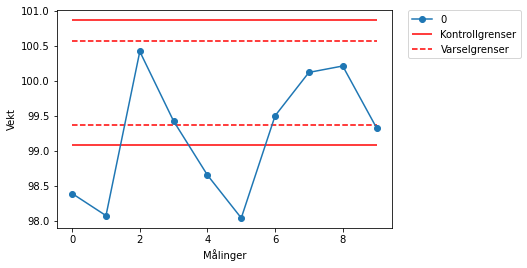
\includegraphics[scale = 0.85]{average.png}
    \caption{Gjennimsnitt av nye målinger med varsel- og kontrollgrenser.\cite{1}}
    \label{fig:fig12}
\end{figure}


Gjennomsnittlig vekt i måling 0, 1, 4 og 5 ligger under kontrollgrensen til Shewhart-diagrammet i \hyperref[fig:fig12]{figur 12}.
Fiskefiletene i disse målingene må derfor ikke sendes ut til kundene.
Måling 9 ligger under varselgrensa og bør sjekkes for individuelle avvik.\\


Ved å lage et s-diagram med kontrollgrenser kan bedriften kontrollere om det opptrer store variasjoner i vekten til de individuelle målingene. Dette gir et mye bedre bilde på vekten til fiskefiletene i hver måling, og kan hjelpe bedriften å komme nærmere en løsning på produksjonsproblemet.

Finner først kvantilene ved hjelp av python og bruker disse til å regne ut øvre- og nedre kontrollgrense for s-diagrammet.
\begin{equation}
    \centering
    \begin{aligned}
    n & = 10\\
    frihetsgrad & = n-1\\\\
     X_{0.002} & = stats.chi2.ppf(0.002, n-1)\\
     X_{0.998} & = stats.chi2.ppf(0.998, n-1)
    \end{aligned}
\end{equation}

Setter kvantilene inn i formlene for øvre- og nedre kontrollgrense ($ØKG_1$ og $NKG_1$.\cite{2}

\begin{equation}
    \centering
\begin{aligned}
\overline{\overline{s_1}} & = 1.951762\\
ØKG_1 & = \overline{\overline{s_1}}*\sqrt{\frac{X_{0.998}}{n-1}}= 4.981433\\
NKG_1 & = \overline{\overline{s_1}}*\sqrt{\frac{X_{0.002}}{n-1}}= 1.142325
\end{aligned}
\end{equation}

\begin{figure}[H]
    \centering
    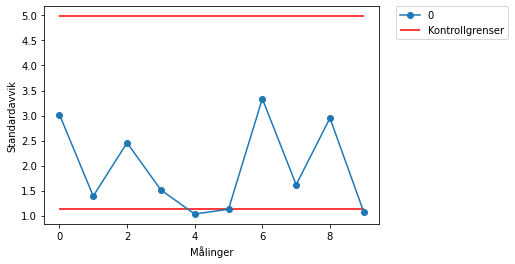
\includegraphics[scale = 0.85]{s_diagram.png}
    \caption{S-diagram med kontrollgrenser}
    \label{fig:fig13}
\end{figure}
I \hyperref[fig:fig13]{figur 13} viser måling 4, 5 og 6 verdier under nedre kontrollgrense. Disse målingene bør derfor fjernes fra distribusjonen.

Gjennomsnittet av standardavvikene ble regnet ut til $\overline{\overline{s_1}}=1.951762$.\\

En butikk som skal kjøpe fisk av bedriften har satt følgende krav som toleransegrense:
\begin{equation}
\begin{aligned}
\centering
&T_U = 103  gram\\
&T_L = 97  gram 
\end{aligned}
\end{equation}

Beregning av kapabilitet og kapabilitetsindeks:
\begin{equation}
\begin{aligned}
 \centering
  &K = 6*\overline{\overline{s_1}}=11.71057\\\\
  &KI = \frac{T_U-T_L}{K}=0.512358\\
\end{aligned}
\end{equation}
Ettersom $KI < 1$ så er kapabiliteten (det området produktene leveres i) større enn det området kunden ønsker produktene i.
Her må det gripes inn for å senke variasjonen, med tanke på at ønskelig tilfelle er $KI > 1$.\cite{3}



\pagebreak
\renewcommand\refname{Referanser}
\begin{thebibliography}{}

\bibitem{Shewhart}
Kjell Arnesen, videoforelesning uke 12.
\textit{Shewhart-diagram.}

\bibitem{s-diagram}
Kjell Arnesen, videoforelesning uke 12.
\textit{s- og p-diagram.}

\bibitem{kapabilitet}
Kjell Arnesen, videoforelesning uke 13.
\textit{Kapabilitet.}


\end{thebibliography}







	
	
	
	
	
	
	
	
\end{document}
